\documentclass[../../../OAE-SPEC-MAIN.tex]{subfiles}
\begin{document}

\section{Flow Transactions}
%\marginnote{See \href{https://en.wikipedia.org/wiki/Ethernet_frame}{Ethernet Frame on Wikipedia}} 

\begin{marginfigure}[-55mm]
  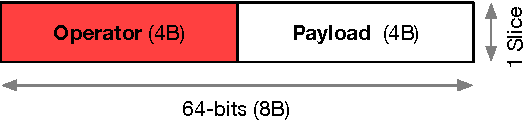
\includegraphics[width=\linewidth]{./figures/1-slice.pdf}
  \caption{1  Slice Flow Subtransaction}
\end{marginfigure}

\begin{marginfigure}[-20mm]
    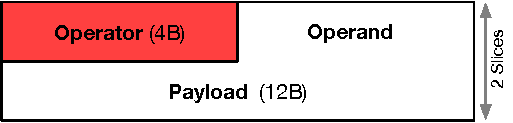
\includegraphics[width=\linewidth]{./figures/2-slice-operator.pdf}
  \caption{2 slice  Flow SubTransaction}% with 12B payload (operand)}
\end{marginfigure}

\begin{marginfigure}
      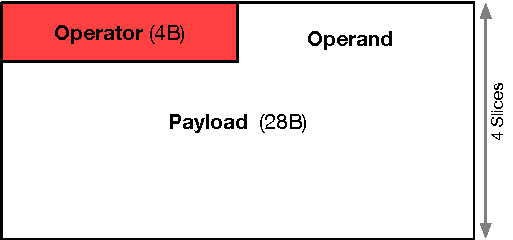
\includegraphics[width=\linewidth]{./figures/4-slice-operator.pdf}
  \caption{4 4 slice Flow SubTransaction with 28B payload (operand) \vspace{15pt}} % TODO Extraneous vspace. Need to eliminate
\end{marginfigure}

\begin{marginfigure}
        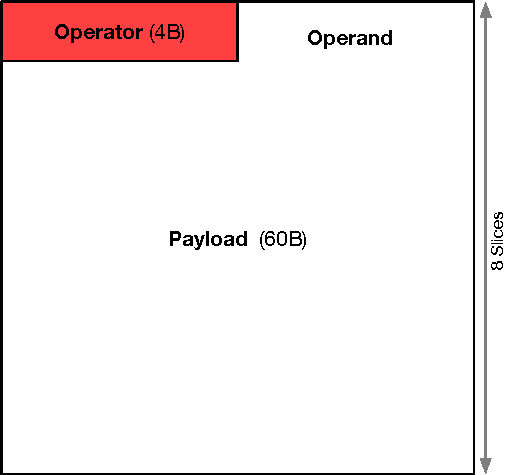
\includegraphics[width=\linewidth]{./figures/8-slice-operator.pdf}
  \caption{1 $\times$ 8 slice Flow  Transaction with 60B payload}
\end{marginfigure}

ULL protocol designers play around with 32 bits as the minimum unit of transactional transfer, but experiments demonstrate the difficulty of making this consistently reliable i; the general consensus is that modern SerDes' work best with $\ge 64$ bit (8 Byte) slices/flits.
%Google Aquila, uses 16 byte flits.
Ethernet  has a minimum frame size of 64 bytes  (although only 42 bytes were available for the payload).

We therefore choose a \emph{fixed} 64 Byte frame for the Shannon Slots, but make them \emph{pre-emptable} so that even the minimum size frame does not need to occupy space on the wire, increase latency, or FPGA processing steps, when the receiver has something more important it wishes to send (e.g. local status messages sent in the background can be pre-empted, giving way to a two phase commit (2PC) transaction).



Some transactional systems are sensitive to making transactions reliable, but don't mind missing events, such as highly perishable market data.  We might call these one-phase commit (1PC) transactions. These can be made to flow at maximum line rate, even though each individual slice is being acknowledged. This is particularly important in HFT for example.

We therefore provide the following ``flow" transactions in the encoding scheme:



% Reference Vortex by Ken Birman

\subsection{Flow Unit Encodings}

\begin{marginfigure}[-10mm]
  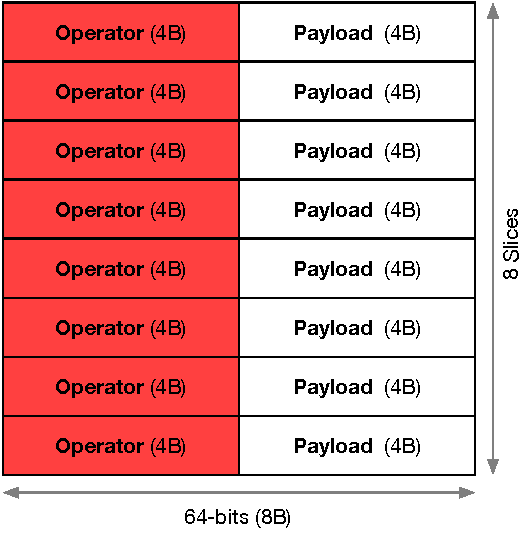
\includegraphics[width=\linewidth]{./figures/8-slices.pdf}
  \caption{8 independent Flow Transactions in a one frame}
  \vspace{8pt}
\end{marginfigure}

\begin{marginfigure}
  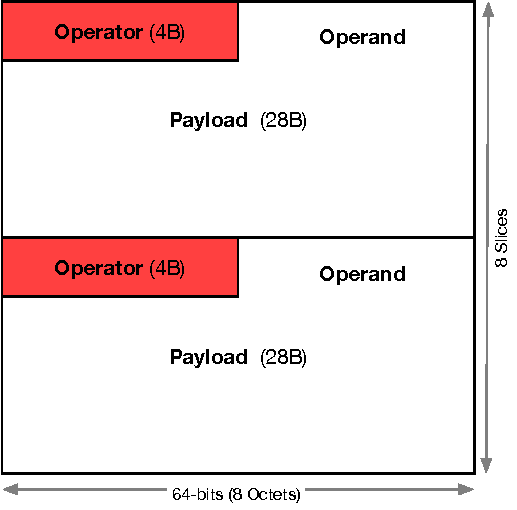
\includegraphics[width=\linewidth]{./figures/2-flow-subtransactions.pdf}
  \caption{2 $\times$ 4 slice Flow Transactions }
  \vspace{8pt}
\end{marginfigure}

\begin{marginfigure}
  \includegraphics[width=\linewidth]{./figures/4-flow-subtransactions.pdf}
  \caption{4 $\times$ 2 slice Flow Transactions}
  \vspace{8pt}
\end{marginfigure}

\begin{marginfigure}
  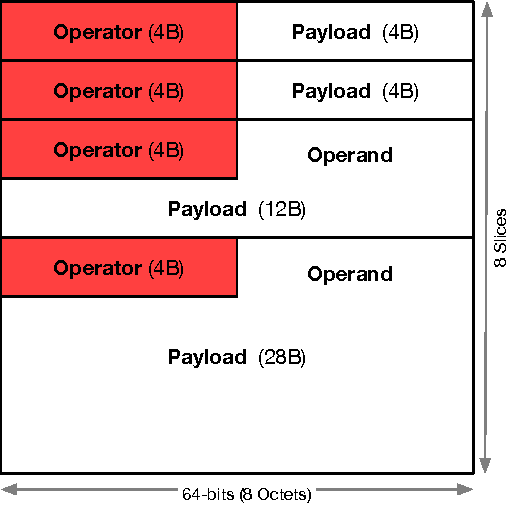
\includegraphics[width=\linewidth]{./figures/Mixed-1-2-4-slice-flowtransactions.pdf}
  \caption{1 64 Byte frame with differently sized flow units}
  \vspace{8pt}
\end{marginfigure}

%* Modeled on the 2SVF

%This encoding scheme (with slice acknowledgements), guarantees common knowledge in a flow of transactions, and their backpropagation packed into a single frame. Examples shown here include:

To enable ultra-low-latency transaction processing, the receiver must begin interpreting and dispatching semantic units (operator + operand) before the full 64-byte frame has arrived. This is made possible through lightweight inline encodings that declare, in the first slice of a transaction, the total number of slices that comprise that flow unit.

These encodings allow the receiver to pipeline semantic processing based on declared intent rather than full-frame arrival, dramatically reducing end-to-end transaction latency while preserving reliability.

%\end{description}


\begin{enumerate}
  \item \textbf{One 1-slice Flow Unit (4B payload)} \\
  \texttt{00} Indicates this flow unit consists of 1 slice.

  \item \textbf{One 2-slice Flow Unit (12B payload)} \\
  \texttt{01} Indicates 2 slices are part of this flow unit. The receiver counts down remaining slices before handoff.

  \item \textbf{One 4-slice Flow Unit (28B payload)} \\
  \texttt{10} Indicates 4 slices make up this flow unit. The receiver pipelines semantic interpretation during arrival.

  \item \textbf{One 8-slice Flow Unit (60B total payload)} \\
  \texttt{11} Indicates 8 slices make up this flow unit. The receiver waits for the full frame before semantic interpretation.
\end{enumerate}

\subsection{Mixing and Matching Flow Transactions}

%\subsection{Two 4 slice Flow Transactions}

You can also mix them in the same frame, but remember, they can only be used for One-Phase-Commit (1PC) in a single stream of transactions. This is because 1PC requires only one "round trip", whereas 2PC requires two round trips (although this scheme can be made to work for 2PC, and perhaps 4PC, but they have not yet been tested).

 
%\subsection{Four  2 slice Flow Transactions}

%\begin{marginfigure}
%        \includegraphics[width=\linewidth]{.././figures/4-flow-subtransactions.pdf}
%  \caption{4 $\times$ 2 slice Flow Subtransaction}
%\end{marginfigure}
%

%\subsection{Eight one-slice  Flow Transactions} 

%\begin{marginfigure} % This is already on the previous page
%        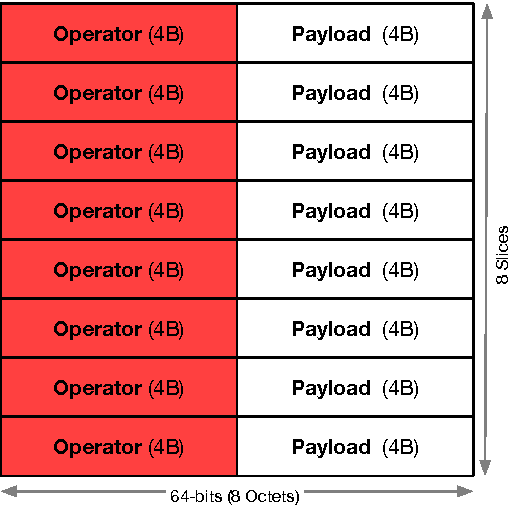
\includegraphics[width=\linewidth]{.././figures/8-flow-subtransactions.pdf}
%  \caption{8 $\times$ 1 slice Flow Transactions}
%\end{marginfigure}



%\subsection{Mixture of different  Flow Transactions} 

%[TESTING TO SEE IF FIGURES IN MARGIN SPREAD OUT CORRECTLY]


%\subsection{Link Efficiency}
% SAHAS - moved table to main column to make it visible.
\begin{table}[ht]
\centering
\caption{Transaction efficiency by operator and operand size.}
\label{tab:txn-efficiency}

\footnotesize
\setlength{\tabcolsep}{3pt} % Tighten column padding
\begin{tabular}{@{}r r r r@{}}
\toprule
Flows & Operator & Operand & Efficiency \\ \midrule
1 & 4 & 4  & 50\%   \\
1 & 4 & 12 & 75\%   \\
1 & 4 & 28 & 87.5\% \\
1 & 4 & 60 & 93.75\%\\
2 & 4 & 4  & 100\%  \\
2 & 4 & 12 & 150\%  \\
2 & 4 & 28 & 175\%  \\
2 & 4 & 60 & 187.5\%\\
4 & 4 & 4  & 200\%  \\
4 & 4 & 12 & 300\%  \\
4 & 4 & 28 & 350\%  \\
4 & 4 & 60 & 375\%  \\
8 & 4 & 4  & 400\%  \\
8 & 4 & 12 & 600\%  \\
8 & 4 & 28 & 700\%  \\
8 & 4 & 60 & 750\%  \\ \bottomrule
\end{tabular}
\end{table}





\end{document}
